% ========================================
%	Header einbinden
% ========================================

\documentclass[bibtotoc,titlepage]{scrartcl}

% Deutsche Spracheinstellungen
\usepackage[ngerman,german]{babel, varioref}
\usepackage[T1]{fontenc}
\usepackage[utf8]{inputenc}

%\usepackage{marvosym}

\usepackage{amsfonts}
\usepackage{amssymb}
\usepackage{amsmath}
\usepackage{amscd}
\usepackage{amstext}

\usepackage{longtable}

%\usepackage{bibgerm}

\usepackage{footnpag}

\usepackage{ifthen}                 %%% package for conditionals in TeX
\usepackage[amssymb]{SIunits}
%Für textumflossene Bilder und Tablellen
%\usepackage{floatflt} - veraltet

%Für Testzwecke aktivieren, zeigt labels und refs im Text an.
%\usepackage{showkeys}

% Abstand zwischen zwei Absätzen nach DIN (1,5 Zeilen)
% \setlength{\parskip}{1.5ex plus0.5ex minus0.5ex}

% Einrückung am Anfang eines neuen Absatzes nach DIN (keine)
%\setlength{\parindent}{0pt}

% Ränder definieren
% \setlength{\oddsidemargin}{0.3cm}
% \setlength{\textwidth}{15.6cm}

% bessere Bildunterschriften
%\usepackage[center]{caption2}


% Problemlösungen beim Umgang mit Gleitumgebungen
\usepackage{float}

% Nummeriert bis zur Strukturstufe 3 (also <section>, <subsection> und <subsubsection>)
%\setcounter{secnumdepth}{3}

% Führt das Inhaltsverzeichnis bis zur Strukturstufe 3
%\setcounter{tocdepth}{3}
\usepackage[version=3]{mhchem}
	\mhchemoptions{minus-sidebearing-left=0.06em, minus-sidebearing-right=0.11em}
\usepackage{exscale}

\newenvironment{dsm} {\begin{displaymath}} {\end{displaymath}}
\newenvironment{vars} {\begin{center}\scriptsize} {\normalsize \end{center}}


\newcommand {\en} {\varepsilon_0}               % Epsilon-Null aus der Elektrodynamik
\newcommand {\lap} {\; \mathbf{\Delta}}         % Laplace-Operator
\newcommand {\R} { \mathbb{R} }                 % Menge der reellen Zahlen
\newcommand {\e} { \ \mathbf{e} }               % Eulersche Zahl
\renewcommand {\i} { \mathbf{i} }               % komplexe Zahl i
\newcommand {\N} { \mathbb{N} }                 % Menge der nat. Zahlen
\newcommand {\C} { \mathbb{C} }                 % Menge der kompl. Zahlen
\newcommand {\Z} { \mathbb{Z} }                 % Menge der kompl. Zahlen
\newcommand {\limi}[1]{\lim_{#1 \rightarrow \infty}} % Limes unendlich
\newcommand {\sumi}[1]{\sum_{#1=0}^\infty}
\newcommand {\rot} {\; \mathrm{rot} \,}         % Rotation
\newcommand {\grad} {\; \mathrm{grad} \,}       % Gradient
\newcommand {\dive} {\; \mathrm{div} \,}        % Divergenz
\newcommand {\dx} {\; \mathrm{d} }              % Differential d
\newcommand {\cotanh} {\; \mathrm{cotanh} \,}   %Cotangenshyperbolicus
\newcommand {\asinh} {\; \mathrm{areasinh} \,}  %Area-Sinus-Hyp.
\newcommand {\acosh} {\; \mathrm{areacosh} \,}  %Area-Cosinus-H.
\newcommand {\atanh} {\; \mathrm{areatanh} \,}  %Area Tangens-H.
\newcommand {\acoth} {\; \mathrm{areacoth} \,}  % Area-cotangens
\newcommand {\Sp} {\; \mathrm{Sp} \,}
\newcommand {\mbe} {\stackrel{\text{!}}{=}}     %Must Be Equal
\newcommand{\qed} { \hfill $\square$\\}
\renewcommand{\i} {\imath}
\def\captionsngerman{\def\figurename{\textbf{Abb.}}}

%%%%%%%%%%%%%%%%%%%%%%%%%%%%%%%%%%%%%%%%%%%%%%%%%%%%%%%%%%%%%%%%%%%%%%%%%%%%
% SWITCH FOR PDFLATEX or LATEX
%%%%%%%%%%%%%%%%%%%%%%%%%%%%%%%%%%%%%%%%%%%%%%%%%%%%%%%%%%%%%%%%%%%%%%%%%%%%
%%%
\ifx\pdfoutput\undefined %%%%%%%%%%%%%%%%%%%%%%%%%%%%%%%%%%%%%%%%% LATEX %%%
%%%
\usepackage[dvips]{graphicx}       %%% graphics for dvips
\DeclareGraphicsExtensions{.eps,.ps}   %%% standard extension for included graphics
\usepackage[ps2pdf]{thumbpdf}      %%% thumbnails for ps2pdf
\usepackage[ps2pdf,                %%% hyper-references for ps2pdf
bookmarks=true,%                   %%% generate bookmarks ...
bookmarksnumbered=true,%           %%% ... with numbers
hypertexnames=false,%              %%% needed for correct links to figures !!!
breaklinks=true,%                  %%% breaks lines, but links are very small
linkbordercolor={0 0 1},%          %%% blue frames around links
pdfborder={0 0 112.0}]{hyperref}%  %%% border-width of frames
%                                      will be multiplied with 0.009 by ps2pdf
%
\hypersetup{ pdfauthor   = {Hannes Franke; Julius Tilly},
pdftitle    = {V301 Innenwiderstand und Leistungsanpassung}, pdfsubject  = {Protokoll FP}, pdfkeywords = {V301, Innenwiderstand, Leistungsanpassung},
pdfcreator  = {LaTeX with hyperref package}, pdfproducer = {dvips
+ ps2pdf} }
%%%
\else %%%%%%%%%%%%%%%%%%%%%%%%%%%%%%%%%%%%%%%%%%%%%%%%%%%%%%%%%% PDFLATEX %%%
%%%
\usepackage[pdftex]{graphicx}      %%% graphics for pdfLaTeX
\DeclareGraphicsExtensions{.pdf}   %%% standard extension for included graphics
\usepackage[pdftex]{thumbpdf}      %%% thumbnails for pdflatex
\usepackage[pdftex,                %%% hyper-references for pdflatex
bookmarks=true,%                   %%% generate bookmarks ...
bookmarksnumbered=true,%           %%% ... with numbers
hypertexnames=false,%              %%% needed for correct links to figures !!!
breaklinks=true,%                  %%% break links if exceeding a single line
linkbordercolor={0 0 1},
linktocpage]{hyperref} %%% blue frames around links
%                                  %%% pdfborder={0 0 1} is the default
\hypersetup{
pdftitle    = {V301 Innenwiderstand und Leistungsanpassung}, 
pdfsubject  = {Protokoll AP}, 
pdfkeywords = {V301, Innenwiderstand, Leistungsanpassung},
pdfsubject  = {Protokoll AP},
pdfkeywords = {V301, Innenwiderstand, Leistungsanpassung}}
%                                  %%% pdfcreator, pdfproducer,
%                                      and CreationDate are automatically set
%                                      by pdflatex !!!
\pdfadjustspacing=1                %%% force LaTeX-like character spacing
\usepackage{epstopdf}
%
\fi %%%%%%%%%%%%%%%%%%%%%%%%%%%%%%%%%%%%%%%%%%%%%%%%%%% END OF CONDITION %%%
%%%%%%%%%%%%%%%%%%%%%%%%%%%%%%%%%%%%%%%%%%%%%%%%%%%%%%%%%%%%%%%%%%%%%%%%%%%%
% seitliche Tabellen und Abbildungen
%\usepackage{rotating}
\usepackage{ae}
\usepackage{
  array,
  booktabs,
  dcolumn
}
\makeatletter 
  \renewenvironment{figure}[1][] {% 
    \ifthenelse{\equal{#1}{}}{% 
      \@float{figure} 
    }{% 
      \@float{figure}[#1]% 
    }% 
    \centering 
  }{% 
    \end@float 
  } 
  \makeatother 


  \makeatletter 
  \renewenvironment{table}[1][] {% 
    \ifthenelse{\equal{#1}{}}{% 
      \@float{table} 
    }{% 
      \@float{table}[#1]% 
    }% 
    \centering 
  }{% 
    \end@float 
  } 
  \makeatother 
%\usepackage{listings}
%\lstloadlanguages{[Visual]Basic}
%\allowdisplaybreaks[1]
%\usepackage{hycap}
%\usepackage{fancyunits}


% ========================================
%	Angaben für das Titelblatt
% ========================================

\title{Ablenkung eines Elektronenstrahls im E- und B-Feld\\				% Titel des Versuchs 
\large TU Dortmund, Fakultät Physik\\ 
\normalsize Anfänger-Praktikum}

\author{Dimitrios Skodras\\			% Name Praktikumspartner A
{\small \href{dimitrios.skodras@tu-dortmund.de}{dimitrios.skodras@tu-dortmund.de}}	% Erzeugt interaktiven einen Link
\and						% um einen weiteren Author hinzuzfügen
Jan Adam\\					% Name Praktikumspartner B
{\small \href{jan.adam@tu-dortmund.de}{jan.adam@tu-dortmund.de}}		% Erzeugt interaktiven einen Link
}
\date{23.Oktober 2012}				% Das Datum der Versuchsdurchführung

% ========================================
%	Das Dokument beginnt
% ========================================

\begin{document}

% ========================================
%	Titelblatt erzeugen
% ========================================

\maketitle					% Jetzt wird die Titelseite erzeugt

\thispagestyle{empty} 				% Weder Kopfzeile noch Fußzeile
% ========================================
%	Der Vorspann
% ========================================

%\newpage					% Wenn Verzeichnisse auf einer neuen Seite beginnen sollen
%\pagestyle{empty}				% Weder Kopf- noch Fußzeile für Verzeichnisse

\tableofcontents

%\newpage					% eine neue Seite
%\thispagestyle{empty}				% Weder Kopf- noch Fußzeile für Verzeichnisse
%\listoffigures					% Abbildungsverzeichnis

%\newpage					% eine neue Seite
%\thispagestyle{empty}				% Weder Kopf- noch Fußzeile für Verzeichnisse
%\listoftables					% Tabellenverzeichnis
\newpage					% eine neue Seite


% ========================================
%	Kapitel
% ========================================

%\section{Einleitung}				% Bei Bedarf
 

\section{Theorie}
Elektronen sind die kleinsten frei auftretenden Elementarteilchen mit einer Masse von  $9,10938291\cdot10^{-31}$ kg und eine negative Ladung von $1,602\cdot10^{-19}$ C. Makroskopische Körper sind dann geladen, wenn sie einen Überschuss oder Mangel an Elektronen aufweisen und dadurch nach außen nicht mehr elektrisch neutral erscheinen. Daher ist die Ladung eines Elektrons die kleinstmögliche Ladung und wird deshalb auch als Elementarladung $e_0$ bezeichnet.\\
In diesen zwei Versuchen werden beschleunigte Elektronen in den Wirkungsbereich von elektrischen und magnetischen Feldern gebracht und der neue Verlauf ihrer Bahnen untersucht.\\
In elektrischen Feldern erfahren Ladungen die sog. Coulombkraft 
\begin{align}
\vec{F_c}=q\cdot\vec{E}.
\end{align}
Positiv geladene Teilchen werden in Richtung der Feldlinien beschleunigt, während negativ geladene Teilchen in die andere Richtung gezogen werden. Die Coulombkraft ist proportional zur Ladung q des Körpers und zur Feldstärke E des elektrischen Feldes.\\
In magnetischen Feldern wirkt auf bewegte Elektronen zusätzlich die sog. Lorentzkraft
\begin{align}
\vec{F_L}=q\cdot(\vec{v}\times\vec{B}).
\end{align}
Diese wirkt jedoch nur auf bewegte Ladungen und lenkt diese senkrecht zu ihrer bisherigen Bewegung und der Richtung des B-Feldes ab. Die Lorentzkraft ist proportional zur Ladung q des Körpers, zur Feldstärke B des magnetischen Feldes und zur Senkrechtkomponente der Geschwindigkeit v der bewegten Ladung in Bezug auf die Ausrichtung des B-Feldes.\\
In den Versuchen soll die Ablenkung durch die entsprechenden Felder gemessen und mit Hilfe eines Kathodenstrahloszilloskopen die Frequenz einer Wechselspannung bestimmt werden. Desweiteren soll mit einem Helmholtzspulenpaar die Stärke des lokalen Erdmagnetfeldes und der Wert der spezifische Ladung $\frac{e_0}{m_0}$ ermittelt werden.

\section{Aufbau und Formeln}
Zentrales Element der Versuche ist eine Kathodenstrahlröhre, die einen variablen Strom von freien Elektronen erzeugt. 

\begin{figure}[htbp]
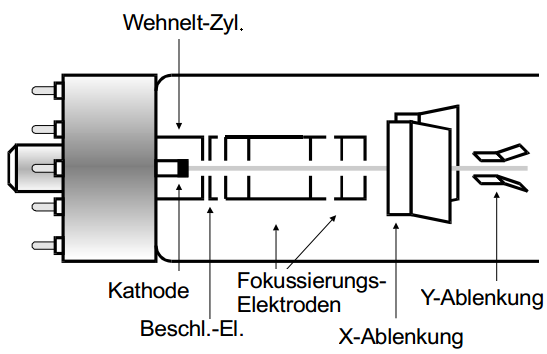
\includegraphics[width=0.6\textwidth] {pics/Kathode.png}
\centering
\caption{Die für beide Versuche verwendete Kathodenstrahlröhre im Querschnitt}
\end{figure}

Die Elektronen treten durch Glühemission aus der passiv geheizten, zylinderförmigen Kathode aus und werden anschließend zur positiv geladenen Anode hin beschleunigt. Die Kathode besteht aus einem Material mit niedriger Elektronenaustrittsarbeit, die durch die Wärmeenergie des Heizdrahtes überwunden wird.
Bevor die Elektronen beschleunigt werden, durchlaufen sie jedoch noch das negative Potential des sog. Wehnelt-Zylinders, wodurch zu langsame Elektronen ausselektiert werden. Hierdurch ist es möglich, die Intensität des Elektronen-Strahls einzustellen.
Nachdem die Elektronen auf ihre Endgeschwindigkeit beschleunigt wurden, wird der Elektronenstrahl durch speziell positionierte inhomogene elektrische Felder fokussiert, bevor er durch die elektrischen Felder zweier Ablenkplattenpaare in x- oder y-Achsenrichtung abgelenkt werden kann.
Der Elektronenstrahl fällt schließlich auf den sog. Leuchtschirm. Dieser ist mit einem speziellen Material bedampft, dessen Aktivatorzentren beim Auftreffen von Elektronen Lichtquanten aussenden und somit den Auftreffpunkt des Elektronenstrahls anzeigen.
Die gesamte Kathodenstrahlröhre muss nahezu vollständig evakuiert sein, da Elektronen selbst mit Luftmolekülen wechselwirken und ansonsten kein unbeeinflusster Elektronenstrahl erzeugt werden könnte. Aus diesem Grund herrscht in der gesamten Kathodenstrahlröhre ein Druck von ca. $10^{-6}$ mbar.

\subsection{Versuch 501: Das elektrische Feld}
Zunächst soll der Einfluss von elektrischen Feldern auf bewegte Elektronen untersucht werden.\\
Umstellen der Energiegleichung $E_{kin}=E_{el}$ nach $v_x$ ergibt
\begin{align} 
v_x&=\sqrt{2\frac{e_0}{m_0}U_b}
\label{vx}
\end{align}
für die Geschwindigkeit $v_x$ des beschleunigten Elektrons.
Die Aufenthaltsdauer des Elektrons im E-Feld der Platten mit der Breite p errechnet sich durch
\begin{align}
\Delta t=\frac{p}{v_x}
\label{deltat}
\end{align}
Auf das Elektron wirkt weiterhin während seiner gesamten Aufenthaltsdauer im homogenen elektrischen Feld die Kraft 
\begin{align}
\vec{F_c}=|e_0\vec{E}|=e_0\frac{U_d}{d}.
\label{Fc}
\end{align}
Teilt man nun \eqref{Fc} durch $m_0$ und integriert über die Aufenthaltsdauer \eqref{deltat}, so ergibt sich für die Geschwindigkeit $v_y$, die das Elektron durch die Ablenkplatten erfährt:
\begin{align}
v_y=\frac{e_0}{m_0}\frac{U_d}{d}\frac{p}{v_x}
\end{align}
Mittels Kleinwinkel-Näherung ergibt sich des weiteren für den Ablenkwinkel $\Theta$
\begin{align*}
tan(\Theta)=\frac{v_y}{v_x}=\frac{e_0}{m_0}\frac{U_d}{d}\frac{p}{v^2_x}=\frac{sin\Theta}{cos\Theta}\cong \Theta
\end{align*}

\begin{figure}[htbp]
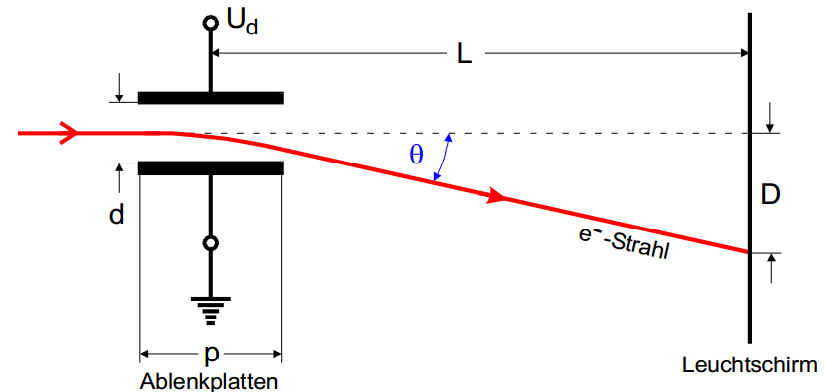
\includegraphics[width=0.7\textwidth] {pics/Ablenkung_E.png}
\centering
\caption{Ablenkung des Elektronenstrahls unter Einwirkung des elektrischen Feldes}
\label{abl_E}
\end{figure}

Einsetzten von \eqref{vx} führt schließlich auf die für die Auswertung benötigte Formel
\begin{align}
D=\frac{p}{2d}L\frac{U_d}{U_B}.
\end{align}

\subsection{Versuch 502: Das magnetische Feld} 
Die Lorentzkraft wirkt nur auf Elektronen, die sich senkrecht zum Magnetfeld bewegen und lenkt diese in eine Richtung senkrecht zur bisherigen Bewegung und senkrecht zum B-Feld ab. Da $\vec{F_L}$ jedoch immer senkrecht auf dem Wegstück $d\vec{s}$ steht, ändert sich die Potentielle Energie des Elektrons nicht. Da Energieerhaltung gilt, muss auch die kinetische Energie
\begin{align*}
E_{kin}=\frac{1}{2}m_0v^2
\end{align*} 
und somit $|\vec{v}|=v_0$ konstant sein.
Ergo ist auch der Radius
\begin{align}
r=\frac{m_0v_0}{e_0B}
\label{r}
\end{align}
konstant und das Elektron beschreibt eine Kreisbahn.

\begin{figure}[htbp]
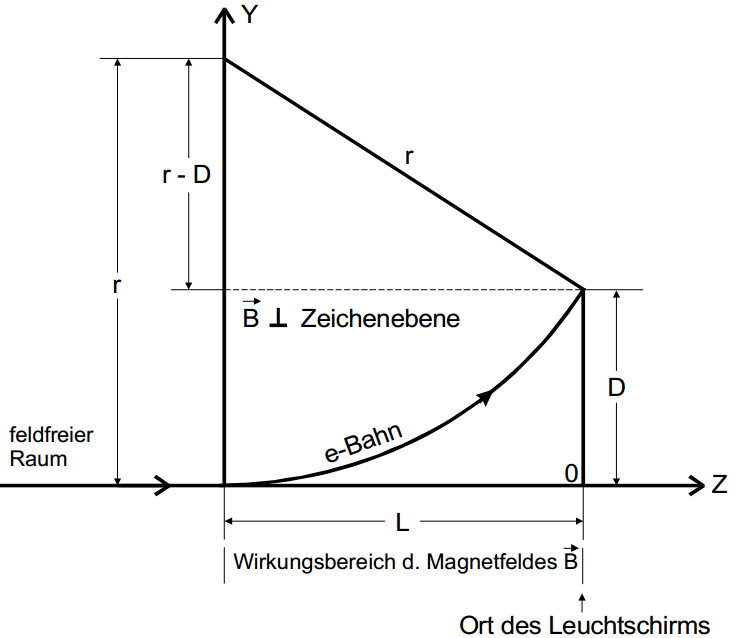
\includegraphics[width=0.6\textwidth]{pics/Ablenkung_B.png}
\centering
\caption{Skizze der Bahnkurve der durch das B-Feld abgelenkten Elektronen und die kennzeichnenden geometrischen Größen}
\label{abl_B}
\end{figure}

Aus Abbildung \eqref{abl_B} kann man durch geometrische Überlegung auf
\begin{align*}
r=\frac{L^2+D^2}{2D}
\end{align*}
für den Radius der Bahnkurve kommen. Einsetzten von Gleichung \eqref{r} und \eqref{vx} führt auf den Ausdruck
\begin{align}
\frac{e_0}{m_0}=\frac{8D^2U_b}{B^2(L^2+D^2)^2}
\label{spezladung}
\end{align}
für die spezifische Ladung $\frac{e_0}{m_0}$.
Die Stärke des B-Feldes der im Versuch genutzten Helmholtzspulen lässt sich berechnen mit
\begin{align}
B=\mu_0 \frac{8}{\sqrt{125}} \frac{NI}{R}.
\label{helmholtz_B}
\end{align}
Die restlichen Größen sind Messwerte oder Kenngrößen der Apparatur.

\section{Durchführung}

\subsection{E-Feld}
Es werden mehrere Messungen der Ablenkung D des Elektronenstrahls in Abhängigkeit der Ablenkspannung $U_d$ durchgeführt, um die Proportionalität zwischen beiden Größen nachzuweisen.
Anschließend wird eine Sinusspannung mit unbekannter Frequenz an die Ablenkplatten in Y-Richtung und eine Sägezahnspannung mit variabler Frequenz an die Ablenkplatte in X-Richtung angeschlossen.
Die Frequenz der Sägezahnspannung wird nun so reguliert, dass sich stehende Lissajou Figuren auf dem Oszilloskop bilden. Die Frequenz der Sinusspannung ist dann ein ganzzahliges Vielfaches der Sägezahnspannung, wodurch ihre Frequenz errechnet werden kann.
\subsection{B-Feld}
Ähnlich wie bei dem elektrischen Feld soll auch die Ablenkung durch das B-Feld untersucht werden. Hierzu erzeugen zwei Helmholtzspulen ein nahezu homogenes Magnetfeld in ihrem Inneren, in welchem sich die Kathodenstrahlröhre befindet. Die gesamte Apparatur wird zunächst so ausgerichtet, dass die Horizontalkomponente des Erdmagnetfeldes in Strahlrichtung zeigt und somit nicht die Elektronen beeinflusst.
Es wird nun eine Messreihe durchgeführt, durch welche der Zusammenhang zwischen der Beschleunigungsspannung $U_b$, der Stärke des B-Feldes der Helmholtzspulen und die Ablenkung D des Elektronenstrahls analysiert, sowie die spezifische Ladung $\frac{e_0}{m_0}$ der Elektronen bestimmt werden soll.\\
Im zweiten Schritt wird der Aufbau senkrecht zum Erdmagnetfeld gedreht, so dass dieses die Elektronen ablenkt. Die Helmholtzspulen werden mit einem Strom betrieben, der ein gerade gleich starkes Gegenfeld erzeugt, so dass die Elektronen wieder zentral auf den Leuchtschirm treffen. Da das B-Feld der Spulen bekannt ist, lässt sich über Winkelbeziehungen die lokale Stärke des Erdmagnetfeldes bestimmen.

\section{Auswertung}

\subsection{Proportionalität zwischen Verschiebung und Ablenkspannung}

\renewcommand{\arraystretch}{1.5}
\begin{table}[htbp]
\begin{tabular}{c|ccccc}
\centering
  & $U_b$ = 225 V &  $U_b$ = 300 V &  $U_b$ = 350 V &  $U_b$ = 400 V &  $U_b$ = 450 V\\
 \hline
 D[cm] & $U_d$[V] & $U_d$[V] & $U_d$[V] & $U_d$[V] & $U_d$[V]\\
 \hline
-1,429	&-9,08	&-11,98	&-15,2	&-16,9&	-19,9\\
-0,794	&-5,31	&-6,08	&-9,3	&-9,8&	-11,5\\
-0,159	&-0,79	&-0,31	&-2,02	&-1,18&	-2,82\\
0,476	&3,30	&5,35	&4,81	&6,24&	6,57\\
1,111	&7,65	&10,91	&11,31	&13,47&	15,07\\
1,746	&11,70	&16,61	&17,93	&20,9	&23,6\\
2,381	&16,03	&21,9	&24,6	&28,8	&31,5\\
3,016	&20,5	&27,4	&31,0	&35,1	&n.D\\
3,651	&24,1	&32,4	&n.D	&n.D	&n.D\\
 \end{tabular}
\caption{Leuchtfleckverschiebung durch Ablenkspannungen bei verschiedenen Beschleunigungsspannungen}
\label{propud}
\end{table}
\renewcommand{\arraystretch}{1}

Aus Tabelle \eqref{propud} ist ersichtlich, dass die Größen D und $U_d$ linear abhängig sind. Durch lineare Regression, 
ausgeführt mit GNUPLOT ergibt sich die Steigung $a = \frac{D}{U_d}$ für die fünf Beschleunigungsspannungen. Bei 
Gegenüberstellung der Empfindlichkeit $a$ und dem Kehrwert zur jeweiligen Beschleunigungsspannung wird ebenfalls eine
lineare Abhängigkeit deutlich.
\renewcommand{\arraystretch}{1.5}
\begin{table}[htbp]
 \begin{tabular}{c|c|c}
  $\frac{1}{U_b}$[$\frac1V$] & a[$\frac{cm}{V}$] & $\Delta$ a[$\frac{cm}{V}$]\\
  \hline
  $4.444 \cdot 10^{-3}$ & 0,1497 & 0,00102 \\
  $3.333 \cdot 10^{-3}$ & 0,1105 & 0,00184 \\
  $2.857 \cdot 10^{-3}$ & 0,0964 & 0,00095 \\
  $2.500 \cdot 10^{-3}$ & 0,0841 & 0,00078 \\
  $2.222 \cdot 10^{-3}$ & 0,0739 & 0,00085 \\
 \end{tabular}
\label{propua}
\centering
\caption{Empfindlichkeit a gegenüber der inversen Beschleunigungsspannung}
\end{table}
\renewcommand{\arraystretch}{1}

Durch Ausgleichsrechnung zwischen der inversen Beschleunigungsspannung und der Empfindlichkeit lässt sich der 
Proportionalitätsfaktor $c$ bestimmen und ergibt 
\begin{align}
 c = (33,532 \pm 0.120) \text{cm} = 33,532 \cdot (1 \pm 0,00358) \text{cm}
 \label{c}.
\end{align}

\begin{figure}[htbp]
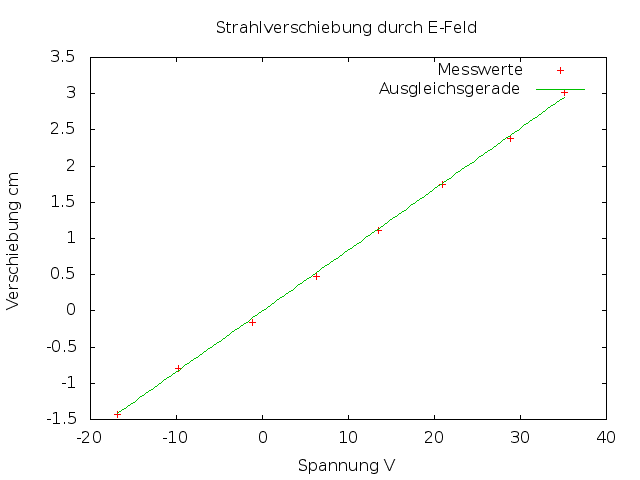
\includegraphics[width=1\textwidth] {pics/400.png}
\centering
\caption{Leuchtfleckverschiebung gegen Ablenkspannung. Hier im Beispiel bei $U_b$ = 400 V}
\end{figure}

\begin{figure}[htb]
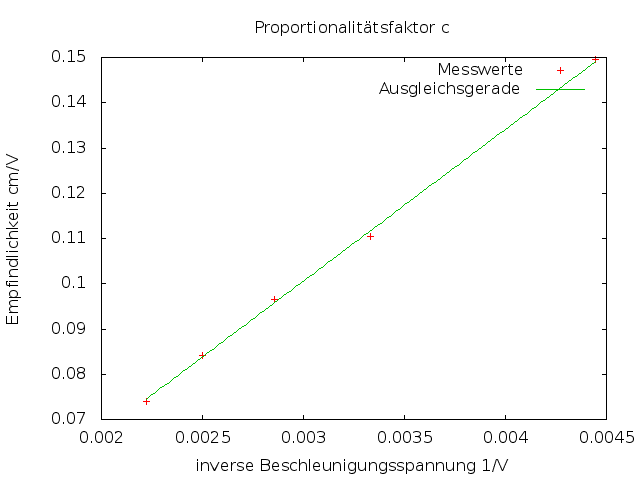
\includegraphics[width=1\textwidth] {pics/proportional.png}
\centering
\caption{Proportionalitätsfaktor c zwischen inverser Beschleunigungsspannung und Empfindlichkeit}
\end{figure}

Der Wert des gewonnenen Faktors $c$ wird nun mit dem gleichbedeutendem $\frac{pL}{2d}$ verglichen.
Aufgrund des veränderlichen Werts für d wird der Mittelwert der Randwerte für d hergenommen.

\begin{align}
 \left< d \right> = \frac{p_1 \cdot d_1 + (p-p_1) \cdot d_2)}{p} = \frac{1,03\text{cm} \cdot 0,38\text{cm} + 0,87\text{cm} \cdot 0,95\text{cm}}{1,9\text{cm}} = 0,64 \text{cm}
\end{align}

somit ergibt sich

\begin{align}
 \frac{pL}{2d} = \frac{1,9\text{cm} \cdot 14,3\text{cm}}{2 \cdot 0,64\text{cm}} = 42,397 \text{cm}.
\end{align}

Die Abweichung vom ermittelten und erwarteten Wert beträgt $\Delta c = \frac{pL}{2d} - c = 8,855 \text{cm}$ und damit ist
c 26,44 \% größer als der Theoriewert.

\subsection{Frequenz des Sinusgenerators}
Durch Variation der Frequenz der Sägezahnspannung $\nu_{Sae}$, welche an das Plattenpaar für die x-Ablenkung angelegt ist,
werden für rationale Verhältnisse zwischen ihr und der zu untersuchenden Sinusspannung stehende Bilder erzeugt.
\renewcommand{\arraystretch}{1.5}
\begin{table}[htbp]
 \centering
\begin{tabular}{c|c|c}
n & $\nu_{Sae}$/Hz & $\nu_{Sin}$/Hz\\
\hline
0.5 & 158,921 & 79,461 \\
1 & 79,472 & 79,472 \\
2 & 39,745 & 79,490 \\
3 & 26,500 & 79,500 \\
\hline
$\left< \nu_{Sin} \right>$ &   & 79,481\\
\end{tabular}
 \caption{Frequenz der Sinusspannung aus Frequenz der Sägezahnspannung und Verhältnis n}
\end{table}
\renewcommand{\arraystretch}{1}

Die beste Schätzfunktion für die Standardabweichung ist gegeben durch

\begin{align}
 S = \sqrt{\frac{1}{N(N-1)} \sum_{k=1}^N (\overline{x} - x_k)^2}
\end{align}

und ergibt für die Frequenz der Sinusspannung einen Wert von \newline
$\nu_{Sin} = (79,481 \pm 0,00877) \text{Hz} = 79,481 \cdot (1 \pm 0,00011) \text{Hz}$.

\subsection{Spezifische Ladung des Elektrons}
Im Folgenden soll durch ein transversales Magnetfeld, erzeugt durch ein Helmholtzspulenpaar (Windungszahl N = 20, Radius R = 0,282m), welches in der Flussdichte B 
veränderlich ist, die spezifische Ladung $\frac{C}{kg}$ des Elektrons ermittelt werden. Entsprechend wird
die gemessene Verschiebung in einen linearisierenden Ausdruck $\rho = \frac{D}{L^2 + D^2}$ mit $L=14,3\text{cm}$, sowie die entsprechende
Stromstärke I in die für die Auswertung relevantere Größe B umgeschrieben.

\renewcommand{\arraystretch}{1.2}
\begin{table}[htbp]
\centering
 \begin{tabular}{c|c|c}
  & $U_b$ = 250 V & $U_b$ = 450 V \\
  \hline
  $\rho$[1/cm] & B[mT] & B[mT]\\
  \hline
  0	&0	&0\\
$3.10\cdot10^{-3}$	&0,019	&0,025\\
$6,16\cdot10^{-3}$	&0,038	&0,053\\
$9,15\cdot10^{-3}$	&0,058	&0,076\\
$12,04\cdot10^{-3}$	&0,076	&0,103\\
$14,80\cdot10^{-3}$	&0,097	&0,130\\
$17.40\cdot10^{-3}$	&0,115	&0,156\\
$19,82\cdot10^{-3}$	&0,139	&0,180\\
$22,06\cdot10^{-3}$	&0,156	&0,207\\
 \end{tabular}
 \caption{Verschiebung D durch das von der Stromstärke induzierte Magnetfeld}
\end{table}
\renewcommand{\arraystretch}{1}

\begin{figure}[htbp]
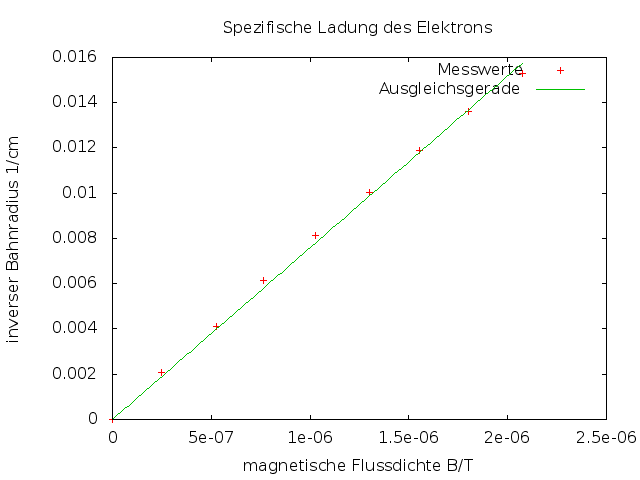
\includegraphics[width=1\textwidth] {pics/spezLadung.png}
\centering
\caption{Proportionalitätsfaktor c zwischen inverser Beschleunigungsspannung und Empfindlichkeit}
\end{figure}

Ausgleichsrechnungen durch GNUPLOT ergeben folgende Faktoren:

\begin{align}
& c_{250} = \frac{\rho}{B} = (10061 \pm 109) \text{Tm} = 10061\cdot(1 \pm 0,011) \text{Tm} \\
& c_{450} = \frac{\rho}{B} = (7593,58 \pm 66,56) \text{Tm} = 7593,58\cdot(1 \pm 0,0088) \text{Tm} 
\end{align}

Nun lässt sich endlich die spezifische Ladung des Elektrons über die Beziehung \eqref{spezladung} ausdrücken.

\begin{align}
\nonumber
\frac{e_0}{m_0}_{250} &= \left( \frac{D \sqrt{8\cdot U_{250}}}{(L^2+D^2)\cdot B} \right)^2 = (c_{250} \sqrt{8\cdot 250 V})^2 = 2,0245 \cdot 10^{11} \frac{C}{kg} \\
 \nonumber
 \frac{e_0}{m_0}_{450} &= \left( \frac{D \sqrt{8\cdot U_{450}}}{(L^2+D^2)\cdot B} \right)^2 = (c_{450} \sqrt{8\cdot 450 V})^2 = 2,0759 \cdot 10^{11} \frac{C}{kg} \\
 \left< \frac{e_0}{m_0} \right> &= 2,0502 \cdot 10^{11} \frac{C}{kg}
\end{align}

Die Abweichung vom Literaturwert\footnote{Steinhäuser, Niko (2003):Die Spezifische Ladung eines Elektrons} beträgt
\begin{align*}
\Delta \frac{e_0}{m_0} = 2,0502 \cdot 10^{11} \frac{C}{kg} - 1,7588 \cdot 10^{11} \frac{C}{kg} = 0,2914 \cdot 10^{11} \frac{C}{kg}
\end{align*}
und liegt damit 16,67 \% darüber.

\subsection{lokale magnetische Flussdichte des Erdmagnetfelds}
Nach der Drehung des Helmholtzspulenpaars um $90^\circ$ im Uhrzeigersinn ist der Leuchtfleck durch das Erdmagnetfeld
von der Stelle (0|0) auf (0|-0,635cm) gewandert. Zur Kompensation ist eine Stromstärke von $I_{Komp} = 240$ mA nötig.
Weiterhin ließ sich der Wert des Inklinationswinkels $\varphi$ = $77^\circ$ durch einen Kompass ermitteln.\\
Aus Gleichung \eqref{helmholtz_B} lässt sich somit die Stärke des durch die Helmholtzspulen erzeugten Gegenfeldes berechnen:
\begin{align}
 \nonumber
 B_{Helmholtz} = B_{hor}= 15,3 \mu\text{T}
 \end{align}
 
Um den Wert des gesamten Magnetfelds an Ort und Zeit des Versuchs zu erhalten, benötigen wir noch die Cosinusbeziehung.

\begin{align}
 B_{hor} = B \cos(\varphi) \Leftrightarrow B = \frac{15,3 \mu\text{T}}{\cos(77^\circ)} = 68,0 \mu\text{T}
\end{align}

\section{Diskussion}
\subsection{Proportionalitätsfaktor c}
Die Abweichung von 26,44\% lässt sich zum Einen sicherlich durch Ungenauigkeit bei der Aufnahme der Messwerte erklären.
So ist die Verschiebung D durch Augenmaß aufgeführt. Zum anderen ist es für den Messprozess erforderlich, dass im Kathodenstrahlrohr das Vakuum perfekt ist. Möglicherweise ist die Röhre jedoch nicht vollständig evakuiert und es somit zu Abweichungen.
\subsection{Spezifische Ladung}
Der Fehler von 16,67\% hat womöglich seine Ursache darin, dass das Magnetfeld des Helmholtzspulenpaars nicht exakt senkrecht
zum Erdmagnetfeld steht. Der zur Verfügung gestellte Kompass zeigte je nach Positionierung im Raum in verschiedene Richtungen.
Außerdem ist wiedermals zu berücksichtigen, dass die Verschiebungen durch Augenmaß ermittelt sind. Trotz dessen ist der Wert
durchaus akzeptabel.
\subsection{Erdmagnetfeld}
Der Wert von 68 $\mu$T ist verglichen mit einem Referenzwert von 64 $\mu$T\footnote[2]{Balck, F. (2010), Erdmagnetfeld URL: \href{http://www2.pe.tu-clausthal.de/agbalck/biosensor/erdmagnetfeld.htm}{http://www2.pe.tu-clausthal.de/agbalck/biosensor/erdmagnetfeld.htm}} in Mitteleuropa schon nahezu einstimmig.

% ========================================
%	Literaturverzeichnis
% ========================================

%\bibliographystyle{plainnat}			% Bibliographie-Style auswählen
%\bibliography{BIBDATEI}				% Literaturverzeichnis

% ========================================
%	Das Dokument endent
% ========================================

\end{document}
